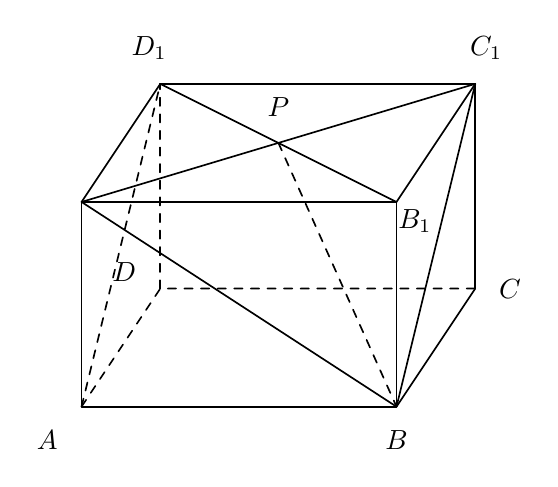
\begin{tikzpicture}[line width=0.6pt,line join=round,line cap=round]
% bottom face: A front-left-bottom, B front-right-bottom, C back-right-bottom, D back-left-bottom
\coordinate (A) at (0,0);
\coordinate (B) at (4,0);
\coordinate (C) at (5.0000000000,1.5000000000);
\coordinate (D) at (1,1.5);
% top face: A1 front-left-top, B1 front-right-top, C1 back-right-top, D1 back-left-top
\coordinate (A1) at (0,2.6);
\coordinate (B1) at (4,2.6);
\coordinate (C1) at (5,4.1);
\coordinate (D1) at (1,4.1);
\coordinate (P) at (2.5,3.35);
% front face solid
\draw (A) -- (B) -- (B1) -- (A1) -- cycle;
% top face solid

\draw (B1) -- (C1);
\draw (C1) -- (D1);
\draw (D1) -- (A1);
% right face solid
\draw (B) -- (C);
\draw (C) -- (C1);
\draw (B) -- (C1);
% left slant solid

% hidden edges meeting at D
\draw[dashed] (A) -- (D) -- (C);
\draw[dashed] (D) -- (D1);
% top diagonals (P is top-face centre, midpoint of B1D1)
\draw (D1) -- (B1);
\draw (A1) -- (C1);
% required segments: PB (interior, hidden) and AD1 (left-face diagonal)
\draw[dashed] (P) -- (B);
\draw[dashed] (A) -- (D1);
% front-face diagonal A1B visible in the original scan
\draw (A1) -- (B);
% labels with clearance
\node[below left=5pt] at (A) {$A$};
\node[below=5pt] at (B) {$B$};
\node[right=5pt] at (C) {$C$};
\node[left=6pt,above=1pt,xshift=-7pt,yshift=-2pt] at (D) {$D$};
\node[left=4pt,above=5pt] at (D1) {$D_{1}$};
\node[right=4pt,above=5pt] at (C1) {$C_{1}$};
\node[right=6pt,xshift=-9pt,yshift=-7pt] at (B1) {$B_{1}$};
\node[above=6pt] at (P) {$P$};
\end{tikzpicture}
